% Options for packages loaded elsewhere
\PassOptionsToPackage{unicode}{hyperref}
\PassOptionsToPackage{hyphens}{url}
%
\documentclass[
]{article}
\usepackage{amsmath,amssymb}
\usepackage{lmodern}
\usepackage{iftex}
\ifPDFTeX
  \usepackage[T1]{fontenc}
  \usepackage[utf8]{inputenc}
  \usepackage{textcomp} % provide euro and other symbols
\else % if luatex or xetex
  \usepackage{unicode-math}
  \defaultfontfeatures{Scale=MatchLowercase}
  \defaultfontfeatures[\rmfamily]{Ligatures=TeX,Scale=1}
\fi
% Use upquote if available, for straight quotes in verbatim environments
\IfFileExists{upquote.sty}{\usepackage{upquote}}{}
\IfFileExists{microtype.sty}{% use microtype if available
  \usepackage[]{microtype}
  \UseMicrotypeSet[protrusion]{basicmath} % disable protrusion for tt fonts
}{}
\makeatletter
\@ifundefined{KOMAClassName}{% if non-KOMA class
  \IfFileExists{parskip.sty}{%
    \usepackage{parskip}
  }{% else
    \setlength{\parindent}{0pt}
    \setlength{\parskip}{6pt plus 2pt minus 1pt}}
}{% if KOMA class
  \KOMAoptions{parskip=half}}
\makeatother
\usepackage{xcolor}
\usepackage[margin=1in]{geometry}
\usepackage{longtable,booktabs,array}
\usepackage{calc} % for calculating minipage widths
% Correct order of tables after \paragraph or \subparagraph
\usepackage{etoolbox}
\makeatletter
\patchcmd\longtable{\par}{\if@noskipsec\mbox{}\fi\par}{}{}
\makeatother
% Allow footnotes in longtable head/foot
\IfFileExists{footnotehyper.sty}{\usepackage{footnotehyper}}{\usepackage{footnote}}
\makesavenoteenv{longtable}
\usepackage{graphicx}
\makeatletter
\def\maxwidth{\ifdim\Gin@nat@width>\linewidth\linewidth\else\Gin@nat@width\fi}
\def\maxheight{\ifdim\Gin@nat@height>\textheight\textheight\else\Gin@nat@height\fi}
\makeatother
% Scale images if necessary, so that they will not overflow the page
% margins by default, and it is still possible to overwrite the defaults
% using explicit options in \includegraphics[width, height, ...]{}
\setkeys{Gin}{width=\maxwidth,height=\maxheight,keepaspectratio}
% Set default figure placement to htbp
\makeatletter
\def\fps@figure{htbp}
\makeatother
\setlength{\emergencystretch}{3em} % prevent overfull lines
\providecommand{\tightlist}{%
  \setlength{\itemsep}{0pt}\setlength{\parskip}{0pt}}
\setcounter{secnumdepth}{5}
\usepackage{booktabs}
\usepackage{longtable}
\usepackage{array}
\usepackage{multirow}
\usepackage{wrapfig}
\usepackage{float}
\usepackage{colortbl}
\usepackage{pdflscape}
\usepackage{tabu}
\usepackage{threeparttable}
\usepackage{threeparttablex}
\usepackage[normalem]{ulem}
\usepackage{makecell}
\usepackage{xcolor}
\ifLuaTeX
  \usepackage{selnolig}  % disable illegal ligatures
\fi
\usepackage[]{natbib}
\bibliographystyle{plainnat}
\IfFileExists{bookmark.sty}{\usepackage{bookmark}}{\usepackage{hyperref}}
\IfFileExists{xurl.sty}{\usepackage{xurl}}{} % add URL line breaks if available
\urlstyle{same} % disable monospaced font for URLs
\hypersetup{
  pdftitle={Assignment},
  pdfauthor={Martijn Koster, 6234119; Jurrian van de Kraats, 5961688; Tim Poorthuis, student nr},
  hidelinks,
  pdfcreator={LaTeX via pandoc}}

\title{Assignment}
\author{Martijn Koster, 6234119 \and Jurrian van de Kraats, 5961688 \and Tim Poorthuis, student nr}
\date{2023-02-15}

\begin{document}
\maketitle

\newpage

\hypertarget{introduction}{%
\section{Introduction}\label{introduction}}

In this paper the

In this paper we will examine whether there is a causal effect from elderly people (i.e., 65+) who have received an influenza vaccine and the likelihood of hospitalization. This will be examined by using the patient records dataset.

Write here a short motivation with a RQ

\begin{itemize}
\tightlist
\item
  well articulated RQ
\end{itemize}

\textbf{The aim of the study is to assess whether annual influenza vaccination reduces the risk of hospitalization among elderly (i.e., people aged \textgreater=65 years).}

\hypertarget{methods}{%
\section{Methods}\label{methods}}

\hypertarget{examening-the-causal-structure}{%
\subsection{Examening the causal structure}\label{examening-the-causal-structure}}

Domain knowledge was used to create a DAG (Figure \ref{fig:dag} ) that explains the causal structure present in the data. The variable `contact with chiropractor' was given as a proxy for the unobserved variable healthy lifestyle. An influenza vaccination is season, hence does the time from last contact with the chiropractor form a causal path to vaccination status. Furthermore is the national distribution of an influenza vaccination determined age, hence does age form a causal path towards vaccination status. Having obtained a influenza vaccination was associated with a lower risk for adverse cardiovascular events with hospitalization as a result \citep{behrouzi}. Having pulmonary disease and diabetes increases ones chances to get severe cardiovascular disease \citep{nhg}. The healthiness of ones lifestyle forms a major cause in getting (severe) cardiovascular disease, pulmonary disease and diabetes. In return is once sex an important confounder in the healthiness of ones lifestyle \citep{loef}. The previously mentioned diseases could all be a cause for hospitalization.\\
The causal paths of the DAG should be examined to asses whether unbiased causal inference is possible. The main two causal paths from vaccination status towards hospitalisation are a direct path and a path through the mediator cardiovascular disease. However, there is a flow of statistical information through open backdoor paths as well. This is due to observed and unobserved confounders like age, contact with chiropractor and healthy lifestyle. The eventual model would need to adjust for these confounders in order to perform an unbiased causal inference.

\begin{figure}
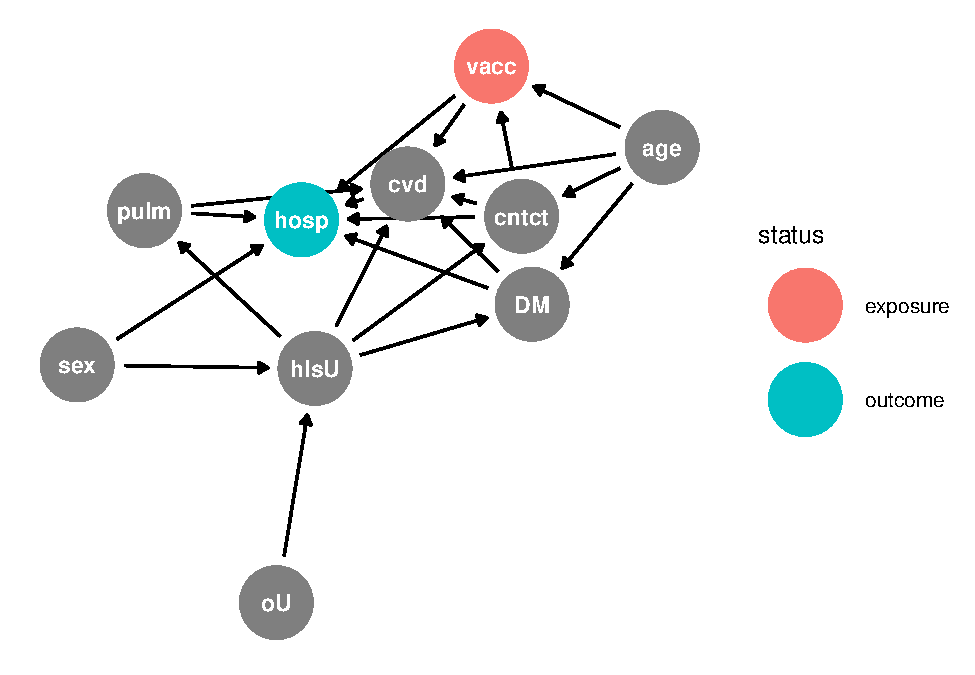
\includegraphics[width=0.5\linewidth]{Assignment_files/figure-latex/dag-1} \caption{DAG model with Vaccine as exposure and hospitalization as outcome}\label{fig:dag}
\end{figure}

\hypertarget{statistical-methods}{%
\subsection{Statistical Methods}\label{statistical-methods}}

\hypertarget{baseline-characteristics}{%
\subsubsection{Baseline Characteristics}\label{baseline-characteristics}}

The electronic patient records dataset consist of eight variables. The variables age and contact with a chiropractor were continues, the variables vaccination status, sex, cardiovascular disease, pulmonary disease, diabetes and hospitalization were binominal. Table \ref{tab:des} presents the baseline characteristics of 40000 individuals who were included in the study. The mean age was 75.65 (sd = 6.97). The majority of the study were woman (61.91\%). Approximately half (49.39\%) of the respondents had Cardiovascular disease, whereas 12.34 percent had Pulmonary disease. Of the participants, 6.54\% had Diabetes Mellitus.\\
\hspace*{0.333em}\hspace*{0.333em}A total of 29616 (74.04\%) respondents were vaccinated. People who received a vaccination had on average more often pulmonary disease (14.33\% vs 6.67\%), cardiovascular disease (53.02\% vs 39.05\%) and diabetes (7.51\% vs 3.8\%).\\
\hspace*{0.333em}\hspace*{0.333em}Baseline characteristics stratified by the study outcome indicate that 254 of the respondents were hospitalized as opposed to 39746 who were not. Respondents who were hospitalized were older (79.68 vs 75.63), had more often contact with the GP (21.08 vs 14.71), were on average less often a female (48.43\% vs 61.99\%), had on average more often cardiovascular disease (72.05\% vs 49.25\%) and on average more often Diabetes (11.42\% vs 6.51\%).

\begin{table}[!h]

\caption{\label{tab:des}Baseline Characteristics stratified by Influenza vaccination received and Hospitalisation}
\centering
\begin{tabular}[t]{llllll}
\toprule
\multicolumn{1}{c}{ } & \multicolumn{1}{c}{ } & \multicolumn{2}{c}{Influenza vaccination received} & \multicolumn{2}{c}{Hospitalized} \\
\cmidrule(l{3pt}r{3pt}){3-4} \cmidrule(l{3pt}r{3pt}){5-6}
Characteristics & Total & Yes & No & Yes & No\\
\midrule
N & 40000 & 29616 & 10384 & 254 & 39746\\
Age, mean (SD) & 75.65 (6.97) & 75.9 (6.83) & 74.97 (7.32) & 79.68 (7.2) & 75.63 (6.97)\\
Contact, mean (SD) & 14.75 (11.54) & 15.85 (11.73) & 11.64 (10.38) & 21.08 (15.59) & 14.71 (11.5)\\
Female, n (\%) & 24763 (61.91) & 18022 (60.85) & 6741 (64.92) & 123 (48.43) & 24640 (61.99)\\
Pulmonary disease, n (\%) & 4937 (12.34) & 4244 (14.33) & 693 (6.67) & 60 (14.33) & 4877 (12.27)\\
\addlinespace
Cardiovascular disease, n (\%) & 19757 (49.39) & 15702 (53.02) & 4055 (39.05) & 183 (72.05) & 19574 (49.25)\\
Diabetes mellitus, n(\%) & 2618 (6.54) & 2223 (7.51) & 395 (3.8) & 29 (11.42) & 2589 (6.51)\\
Received Influenza Vaccination, n (\%) &  &  &  & 184 (72.44) & 29432 (74.05)\\
\bottomrule
\end{tabular}
\end{table}

\hypertarget{propensity-scores-ps}{%
\subsubsection{Propensity Scores (PS)}\label{propensity-scores-ps}}

In order to control for confounding (observed and unobserved), a PS was estimated by fitting a logistic regression. A PS gives the probability being vaccinated for the respondents. The variables used to calculate the propensity score are derived from the aforementioned DAG (Figure \ref{fig:dag} ), namely: age, sex, cardiovascular disease, pulmonary disease, diabetis mellitus, and GP contact in 12 months prior to start of study. For the variables age and contact a spline is used, because showed favorable performance compared to other propensity score methods \citep{Tian}.\\
\hspace*{0.333em}\hspace*{0.333em}\hspace*{0.333em}\hspace*{0.333em}In Figure \ref{fig:psscore}, the PS for vaccinated and unvaccinated individuals appear to be well-balanced, indicating that the distribution of covariates between the two groups is similar. This plot also supports the positivity assumption, which means that both vaccinated and unvaccinated individuals are represented in all sub-populations defined by different combinations of covariates \citep{westreich}.

\hypertarget{ps-as-covariate}{%
\subsubsection{PS as Covariate}\label{ps-as-covariate}}

The first adjusted model is to use the PS as a covariate. In a observational study the treated and untreated group have an equal distribution given that these are divided in groups of a constant propensity. The propensity score can be used as a baseline variable to account for the dimensional difference between groups since it is assumed that the treatment is unconfounded given this propensity score. \citep{schafer}. This method also provides more statistical power and precision than matching, particularly when the sample size is large \citep{austin}.

\hypertarget{inverse-probability-weighting-ipw}{%
\subsubsection{Inverse Probability Weighting (IPW)}\label{inverse-probability-weighting-ipw}}

With the aforementioned propensity scores, IPW is calculated by \(\frac{1}{PS}\) for the vaccinated group and \(\frac{1}{1-PS}\) for the unvaccinated. IPW creates a pseudo-population by replicating observations of individuals with higher weights, so the probability of exposure isn't affected by covariates. For example, if gender affects both exposure and outcome, IPW assigns greater weights to underrepresented groups, achieving a comparable gender ratio between the exposed and unexposed groups in the pseudo-population. This allows for comparison of the weighted outcome averages between the exposed and unexposed individuals in the pseudo-population, with no confounding from measured covariates \citep{shiba}.\\
Two model were created, one with stabilized- and one with unstabilized weights. When using stabilized weights the numerator model also includes confounders, giving more stable estimates compared to the unstabilized weights \citep{ipw}. In both models bootstrapping was used to account for the inflated sample size of the pseudo population.

\begin{figure}
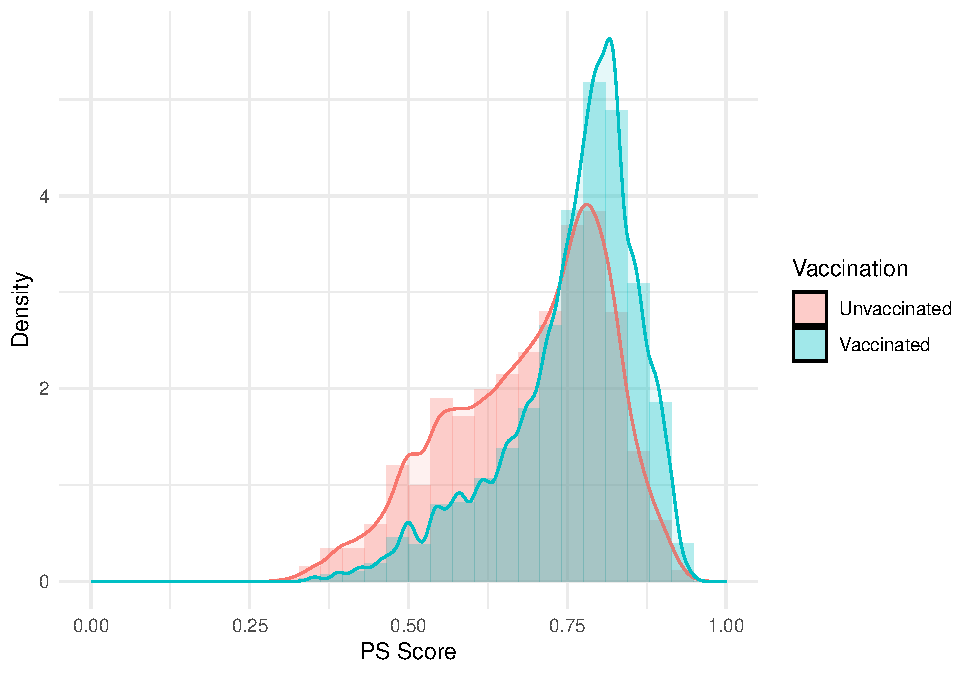
\includegraphics[width=0.7\linewidth]{Assignment_files/figure-latex/psscore-1} \caption{Distribution of the Propensity score for participants who received a vaccination compared with those who did not receive a vaccination}\label{fig:psscore}
\end{figure}

\hypertarget{results}{%
\section{Results}\label{results}}

As shown in Table \ref{tab:res}, the crude association between vaccination status and hospitalization was examined using logistic regression, and the odds ratio was found to be 0.921 (95\% CI: 0.699, 1.214), indicating a non-significant association (p = 0.562). The C-statistic, a measure of discrimination, was 0.508, suggesting poor predictive performance of the model.\\
\hspace*{0.333em}\hspace*{0.333em}\hspace*{0.333em}\hspace*{0.333em}Considering the second model in Table \ref{tab:res}, which presents the PS score as covariate, the Odds Ratio suggests a significant negative association (adjusted OR: 0.635. 95\% CI 0.478 to 0.843; p \textless.001). The C-Statistic of 0.679 suggests that the model has moderate discriminatory power.\\
\hspace*{0.333em}\hspace*{0.333em}\hspace*{0.333em}\hspace*{0.333em}The IPW model with unstabilised weights yields significant negative association between the exposure and outcome variable (adjusted OR: 0.617, 95\%CI 0.523 to 0.728; p \textless.001). The model presents moderate discriminatory power, where C = 0.573.\\
\hspace*{0.333em}\hspace*{0.333em}\hspace*{0.333em}\hspace*{0.333em}The last model in Table \ref{tab:res} is an IPW model with stabilised weights. This model also presents a negative association between vaccination and hospitalisation (Adjusted OR: 0.617, 95\% CI 0.509 to 0.748; p \textless.001). The C-statistic suggests moderate discriminatory power (C= 0.573).

\begin{table}[!h]

\caption{\label{tab:res}Association between influenza vaccination and hospitalization (n=40000)}
\centering
\begin{tabular}[t]{lllr}
\toprule
Model Specification & OR (95\% CI) & P-Value & C-Statistic\\
\midrule
Unadjusted & 0.921 (0.699 to 1.214) & 0.562 & 0.508\\
PS score as covariate & 0.635 (0.478 to 0.843) & <.001 & 0.679\\
Unstabilised IPW & 0.617 (0.523 to 0.728) & <.001 & 0.573\\
Stabilised IPW & 0.617 (0.509 to 0.748) & <.001 & 0.573\\
\bottomrule
\end{tabular}
\end{table}

\hypertarget{conclusion-discussion}{%
\section{Conclusion / Discussion}\label{conclusion-discussion}}

\begin{itemize}
\item
  Conclusions supported by data
\item
  Other issues (both positive and negative) Maybe write something about matching here?
\end{itemize}

  \bibliography{references.bib}

\end{document}
